\section{Can Bus Systeme}
\label{sec:Can_Bus_Controller}

Ein typischer Bereich, in dem die Nutzung von CAN-Bussen unumgänglich ist, wäre die Automobilindustrie. Moderne Auto verfügen Heutzutage über eine Vielzahl an elektronischen Systemen, die miteinander kommunizieren müssen. Und die übliche Verkabelungen wäre mit dem Vielzahl an Steuergeräten kaum mehr möglich. Der CAN-Bus ist in der CAN-Spezifikation von  \cite{Bosch1991} als ein Multicast-Kommunikationsprotokoll definiert, das folgende Vorteile aufweist
\begin{itemize}
	\item CAN ist ein Multi-Master-Broadcast-System. Das heißt, dass jeder Knoten auf dem Bus mit jedem anderen Knoten kommunizieren kann.
	\item Der CAN-Bus hat eine Datenübertragungsgeschwindigkeit von bis zu 1 Mbit/s.
	\item Jeder neue Knoten kann in den Bus eingefügt werden, ohne die ursprüngliche Hardware zu verändern.
	\item Es bietet eine Fehlerprüfung zur Vermeidung von Busfehlern.
	 \item Das differentielle CAN-Signal bietet eine hohe Rauschunterdrückung.
\end{itemize}

Da dieses Protokoll sehr viele Vorteile mitbringt, wurde es in den letzten Jahren in der Industrie sehr viel verbreitet. In viele Mikrocontroller werde auf diesem Grund bei der Herstellung ein CAN-Bus eingebaut.  

%------------Bild einfügen------------
%\begin{figure}
 % \begin{center}
  %  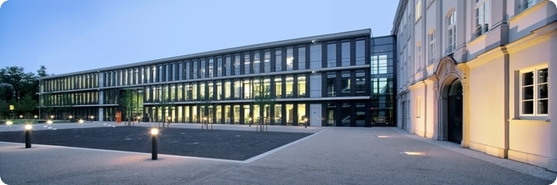
\includegraphics[width=0.6\textwidth]{./images/hochschule.jpg}
  %\end{center}
  %\vspace{-5pt}
  %\caption[Hochschule Augsburg]{Hochschule Augsburg \cite{HSA.2013}} % %Eckige Klammer (optional): Caption-Text in Abbildungsverzeichnis
  %\label{fig:hochschule}
  %\vspace{-5pt}
%\end{figure}

\subsection{Can Message Frame}
\label{subsec:can_bus_controller:can_frame}

In der Sprache des CAN-Standards werden alle Nachrichten als Frames bezeichnet; es gibt Daten-Frames, Remote-Frames, Error-Frames und Overload-Frames. Die an den CAN-Bus gesendeten Informationen müssen definierten Frame-Formaten von unterschiedlicher, aber begrenzter Länge entsprechen.
CAN verfügt über vier verschiedene Arten von Message Frames:

\begin{itemize}
	\item \textbf{Data Frame (Sendet Daten)}: Die Daten werden von einem Sendeknoten zu einem oder mehreren Empfangsknoten übertragen.
	\item \textbf{Remote Frame (Fordert Daten an)}: Jeder Knoten kann Daten von einem Quellknoten anfordern. Auf einen Remote-Frame folgt somit ein Daten-Frame, der die angeforderten Daten enthält
	\item \textbf{Error Frame (Meldet einen Fehlerzustand)}: Jeder Busteilnehmer, egal ob Sender oder Empfänger, kann zu jeder Zeit während einer Daten- oder Remote-Frame-Übertragung einen Fehlerzustand melden.
	\item \textbf{Overload-Frame  (Meldet Knotenüberlastung)}: Ein Knoten kann zwischen zwei Daten- oder Remote-Frames eine Verzögerung anfordern, das heißt, dass der Overload-Frame nur zwischen Daten- oder Remote-Frame-Übertragungen auftreten kann.
\end{itemize}

Im Nachfolgenden gegen wir auf der Architektur von den jeweiligen CAN Frame Typen ein.
\subsubsection{Data Frame}
\begin{figure}[h]
	 \begin{center}
	  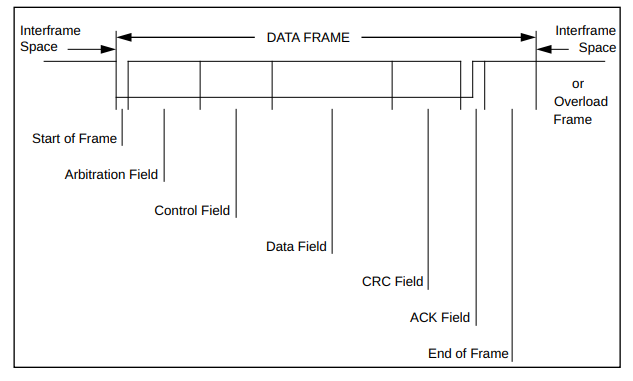
\includegraphics[width=1\textwidth]{./images/CAN-data-frame.jpg}
	\end{center}
	\vspace{-5pt}
	\caption[CAN-Data Frame Architektur]{CAN-Data Frame Architektur \cite{Bosch1991}[p.~12]} % Eckige Klammer (optional): Caption-Text in Abbildungsverzeichnis
	\label{fig:can-data-frame}
	\vspace{-5pt}
	\end{figure}
Die Abbildung ~\ref{fig:can-data-frame} beschreibt die 7 Bestandteile, aus denen ein Data Frame besteht, namlich:
\begin{itemize}
	\item \textbf{SOF}(Start of Frame):  Zeigt den Beginn von Daten und Remote Frames an.
	\item \textbf{Arbitration Field}: der besteht auf
		\begin{itemize}
			\item Identifikator: Die Basis-ID besteht aus 11 Bits und die erweiterte ID aus 29 Bits.
			\item RTR(Remote Transmission Request)-Bit: Im Data Frame ist das RTR-Bit "0". Im RTR-Frame hingegen ist es "1".
		\end{itemize}
	\item \textbf{Control Field}: Dient zur Bestimmung der Datengröße und der Länge der Nachrichten-ID. der besteht auf 6 Bits.
		\begin{itemize}
			\item IDE ( Identifikator-Erweiterung): Dieses Bit bestimmt den Identifikator als Basis-ID oder Erweiterte ID.
			\item R0,R1: reservierte Bits.
			\item DLD (Data Length Code): Er wird zur Bestimmung der Datenlänge verwendet.
		\end{itemize}
	\item \textbf{Data Field}: bis zu 8 Byte Datenfeld.
	\item \textbf{CRC-Field (Cyclic Redundancy Check)}: zur Überprüfung der Datenkorrektur.
	\item \textbf{ACK Field (Acknowledgement Field)}: um zu bestimmen, ob die Nachricht empfangen wurde oder nicht. Bei Empfang von Daten wird dieses Bit auf High gezogen.
	\item \textbf{EOF (End of Frame)}: Zeigt das Ende von Daten- und Remote-Frames an.
\end{itemize}

\subsubsection{Remote Frame}
\begin{figure}[h]
	\begin{center}
		\includegraphics[width=1\textwidth]{./images/CAN-remote-frame.jpg}
	\end{center}
	\vspace{-5pt}
	\caption[CAN-Remote Frame Architektur]{CAN-Remote Frame Architektur \cite{Bosch1991}[p.~17]} % Eckige Klammer (optional): Caption-Text in Abbildungsverzeichnis
	\label{fig:can-remote-frame}
	\vspace{-5pt}
\end{figure}
 Die Abbildung ~\ref{fig:can-remote-frame} beschreibt die Bestandtele einem Remote-Frame. Data-Frame und Remote-Frame sind sich beide sehr ähnlich. Im Prinzip ist der Remote Frame ein Data Frame ohne das Datenfeld. Dieser besteht in der Regel aus den gleichen Bestandteilen wie der Data Frame.
 
 \subsubsection{Error Frame}
 
 Abbildung ~\ref{fig:can-error-frame} zeigt die Struktur der Error Frame an. Der Error Frame besteht aus zwei Teilen:
 \begin{itemize}
 	\item Error Flag: stellt ein Knoten einen Fehlerzustand fest, erzeugt er bis zu 12 Bits "0" für das Fehlerflag.
 	\item Error Delimiter: 8 Bits "1" beenden den Error Frame.
 \end{itemize}
 
 \begin{figure}[h]
 	\begin{center}
 	  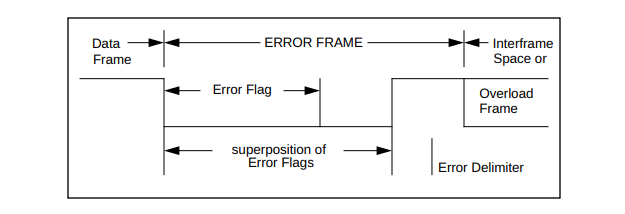
\includegraphics[width=1\textwidth]{./images/Can-error-frame.jpg}
 	\end{center}
 	\vspace{-5pt}
 	\caption[Can-Error-Frame]{Can-Error-Frame \cite{Bosch1991}[p.~18]} % Eckige Klammer (optional): Caption-Text in Abbildungsverzeichnis
 	\label{fig:can-error-frame}
 	\vspace{-5pt}
 \end{figure}

\subsubsection{Overload Frame}
 Abbildung ~\ref{fig:can-overload-frame} ist der Überlastrahmen. Er wird von dem Empfängerknoten erzeugt, um mehr Verzögerung zwischen den Datenrahmen zu erzwingen.

\begin{figure}[h]
	\begin{center}
		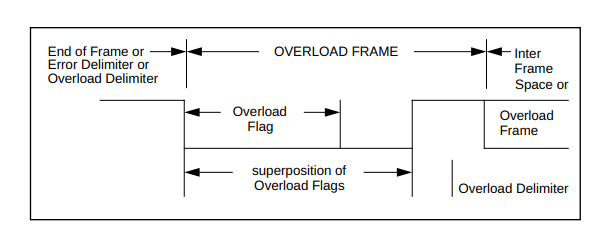
\includegraphics[width=1\textwidth]{./images/Can-overload-frame.jpg}
	\end{center}
	\vspace{-5pt}
	\caption[Can-Overload-Frame]{Can-Overload-Frame \cite{Bosch1991}[p.~19]} % Eckige Klammer (optional): Caption-Text in Abbildungsverzeichnis
	\label{fig:can-overload-frame}
	\vspace{-5pt}
\end{figure}



%\paragraph*{Beispiel}-----------Paragraph erstellen
%------------------- wrapfigure einfügen----------------------
%\begin{wrapfigure}{r}{0.45\textwidth}
 % \vspace{-20pt}
  %\begin{center}
  %  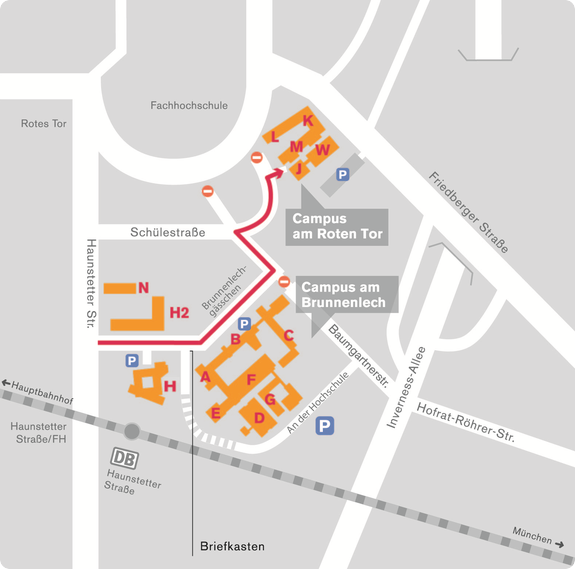
\includegraphics[width=0.45\textwidth]{./images/standort_rotes_tor_anfahrt_klm_bau.png}
  %\end{center}
  %\vspace{-20pt}
  %\caption[Standort Rotes Tor]{Standort Rotes Tor \cite{HSA.2013}}
  %\label{fig:standort_rotes_tor_anfahrt_klm_bau}
  %\vspace{-10pt}
%\end{wrapfigure}

\subsection{Can Physical Layer}
\label{subsec:can_bus_controller:can_physical_layer}
Der CAN FD Protokoll, der während dieser Arbeit verwendet wird, ist in ISO 1189-1:2015 definiert. Dieses Protokoll beschreibt nicht die mechanischen, Drähte, und Anschlüsse, aber fordert allerdings, dass die Drähte und Anschlüsse den elektrischen Spezifikationen entsprechen müssen. 
\begin{figure}[h]
	\begin{center}
		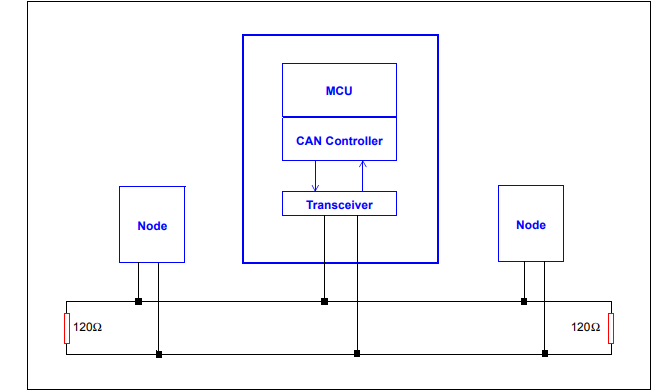
\includegraphics[width=1\textwidth]{./images/Can-connexion.jpg}
	\end{center}
	\vspace{-5pt}
	\caption[Can-Bus Connexion]{Can-Bus Connexion \cite{Richards2002}[p.~2]} % Eckige Klammer (optional): Caption-Text in Abbildungsverzeichnis
	\label{fig:can-bus-connexion}
	\vspace{-5pt}
\end{figure}
Abbildung ~\ref{fig:can-bus-connexion} zeigt eine CAN-Verbindung mit zwei CAN-Node gemäß der ISO-11898-1 CAN-Spezifikation. CAN High(CAN_H) und CAN Low(CAN_L) verlangen zwei 120\si{\ohm}-Abschlusswiderstände. Der Transceiver wandelt die von CAN-Knoten kommenden CAN-Signale in ein digitales Rx- und Tx-Signal für den Node Controller um.
Des Weiteren handelt es sich bei CAN_H und CAN_L um Differenzsignale. wie auf der Abbildung  ~\ref{fig:can-h:can-l}  zu sehen ist, wenn die zwei Signale bei 2,5 V liegen, ist dies ein rezessives Signal, also eine logische 0. Wenn CAN_H auf 3,5 V und CAN_L auf auf 1,5 V, dann handelt es sich um ein dominantes Signal, also eine logische 1. 
\begin{figure}[h]
	\begin{center}
		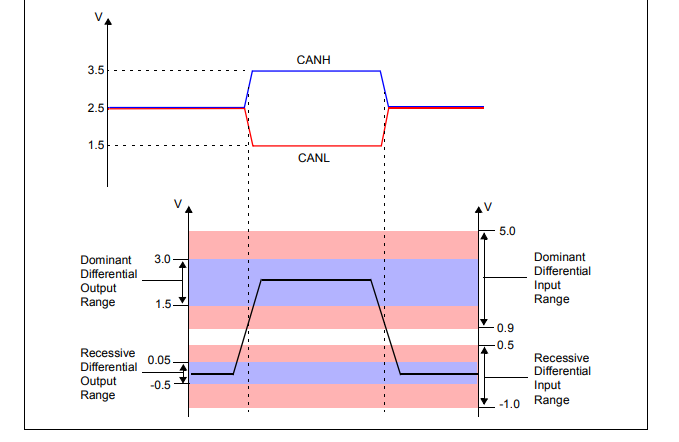
\includegraphics[width=1\textwidth]{./images/can-high-low.jpg}
	\end{center}
	\vspace{-5pt}
	\caption[CAN_H and CAN_L]{CAN_H and CAN_L \cite{Richards2002}[p.~3]} % Eckige Klammer (optional): Caption-Text in Abbildungsverzeichnis
	\label{fig:can-h:can-l}
	\vspace{-5pt}
\end{figure}